%% abtex2-modelo-relatorio-tecnico.tex, v-1.9.7 laurocesar
%% Copyright 2012-2018 by abnTeX2 group at http://www.abntex.net.br/ 
%%
%% This work may be distributed and/or modified under the
%% conditions of the LaTeX Project Public License, either version 1.3
%% of this license or (at your option) any later version.
%% The latest version of this license is in
%%   http://www.latex-project.org/lppl.txt
%% and version 1.3 or later is part of all distributions of LaTeX
%% version 2005/12/01 or later.
%%
%% This work has the LPPL maintenance status `maintained'.
%% 
%% The Current Maintainer of this work is the abnTeX2 team, led
%% by Lauro César Araujo. Further information are available on 
%% http://www.abntex.net.br/
%%
%% This work consists of the files abntex2-modelo-relatorio-tecnico.tex,
%% abntex2-modelo-include-comandos and abntex2-modelo-references.bib
%%

% ------------------------------------------------------------------------
% ------------------------------------------------------------------------
% abnTeX2: Modelo de Relatório Técnico/Acadêmico em conformidade com 
% ABNT NBR 10719:2015 Informação e documentação - Relatório técnico e/ou
% científico - Apresentação
% ------------------------------------------------------------------------ 
% ------------------------------------------------------------------------

\documentclass[
	% -- opções da classe memoir --
	12pt,				% tamanho da fonte
	openright,			% capítulos começam em pág ímpar (insere página vazia caso preciso)
	oneside,			% para impressão em recto e verso. Oposto a oneside
	a4paper,			% tamanho do papel. 
	% -- opções da classe abntex2 --
	%chapter=TITLE,		% títulos de capítulos convertidos em letras maiúsculas
	%section=TITLE,		% títulos de seções convertidos em letras maiúsculas
	%subsection=TITLE,	% títulos de subseções convertidos em letras maiúsculas
	%subsubsection=TITLE,% títulos de subsubseções convertidos em letras maiúsculas
	% -- opções do pacote babel --
	english,			% idioma adicional para hifenização
	french,				% idioma adicional para hifenização
	spanish,			% idioma adicional para hifenização
	brazil,				% o último idioma é o principal do documento
	]{abntex2}


% ---
% PACOTES
% ---

% ---
% Pacotes fundamentais 
% ---
\usepackage{lmodern}			% Usa a fonte Latin Modern
\usepackage[T1]{fontenc}		% Selecao de codigos de fonte.
\usepackage[utf8]{inputenc}		% Codificacao do documento (conversão automática dos acentos)
\usepackage{indentfirst}		% Indenta o primeiro parágrafo de cada seção.
\usepackage{color}				% Controle das cores
\usepackage{graphicx}			% Inclusão de gráficos
\usepackage{microtype} 			% para melhorias de justificação
\usepackage{pdfpages}
\usepackage{lscape}
\usepackage{tikz}
\usepackage{geometry}
\usepackage{pdflscape}
\usetikzlibrary{shapes.gates.logic.US,trees,positioning,arrows}
\newcommand{\under}{\underline{ }}
\usetikzlibrary{arrows,automata}
\usetikzlibrary{positioning}
\usepackage{tikz-uml}
% ---
% Pacotes adicionais, usados no anexo do modelo de folha de identificação
% ---
\usepackage{multicol}
\usepackage{multirow}
% ---
	
% ---
% Pacotes adicionais, usados apenas no âmbito do Modelo Canônico do abnteX2
% ---
\usepackage{lipsum}				% para geração de dummy text
% ---

% ---
% Pacotes de citações
% ---
\usepackage[brazilian,hyperpageref]{backref}	 % Paginas com as citações na bibl
\usepackage[alf]{abntex2cite}	% Citações padrão ABNT

% --- 
% CONFIGURAÇÕES DE PACOTES
% --- 

% ---
% Configurações do pacote backref
% Usado sem a opção hyperpageref de backref
\renewcommand{\backrefpagesname}{Citado na(s) página(s):~}
% Texto padrão antes do número das páginas
\renewcommand{\backref}{}
% Define os textos da citação
\renewcommand*{\backrefalt}[4]{
	\ifcase #1 %
		Nenhuma citação no texto.%
	\or
		Citado na página #2.%
	\else
		Citado #1 vezes nas páginas #2.%
	\fi}%
% ---

% ---
% Informações de dados para CAPA e FOLHA DE ROSTO
% ---
\titulo{Proposta de modelagem de banco de dados NoSQL}
\autor{Vanessa Martinez Tonini}
\local{São Paulo}
\data{2019}
\instituicao{%
  Universidade de São Paulo -- USP
  \par
  Instituto de Matemática e Estatística
  \par
  Programa de Pós-Graduação}
\tipotrabalho{Exercício}
% O preambulo deve conter o tipo do trabalho, o objetivo, 
% o nome da instituição e a área de concentração 
\preambulo{Trabalho apresentado para a disciplina MAC5861 – Modelagem de Banco de Dados. Proposta de modelagem para uma banco de dados NoSQL baseado no modelo de dados de agregados. }
\orientador{Profª. Kelly Rosa Braghetto}
% ---
 
% ---
% Configurações de aparência do PDF final

% alterando o aspecto da cor azul
\definecolor{blue}{RGB}{41,5,195}

% informações do PDF
\makeatletter
\hypersetup{
     	%pagebackref=true,
		pdftitle={\@title}, 
		pdfauthor={\@author},
    	pdfsubject={\imprimirpreambulo},
	    pdfcreator={LaTeX with abnTeX2},
		pdfkeywords={abnt}{latex}{abntex}{abntex2}{relatório técnico}, 
		colorlinks=true,       		% false: boxed links; true: colored links
    	linkcolor=blue,          	% color of internal links
    	citecolor=blue,        		% color of links to bibliography
    	filecolor=magenta,      		% color of file links
		urlcolor=blue,
		bookmarksdepth=4
}
\makeatother
% --- 

% --- 
% Espaçamentos entre linhas e parágrafos 
% --- 

% O tamanho do parágrafo é dado por:
\setlength{\parindent}{1.3cm}

% Controle do espaçamento entre um parágrafo e outro:
\setlength{\parskip}{0.2cm}  % tente também \onelineskip

% ---
% compila o indice
% ---
\makeindex
% ---

% ----
% Início do documento
% ----
\begin{document}


% Seleciona o idioma do documento (conforme pacotes do babel)
%\selectlanguage{english}
\selectlanguage{brazil}

% Retira espaço extra obsoleto entre as frases.
\frenchspacing 

% ----------------------------------------------------------
% ELEMENTOS PRÉ-TEXTUAIS
% ----------------------------------------------------------
% \pretextual

% ---
% Capa
% ---
\imprimircapa
% ---

% ---
% Folha de rosto
% (o * indica que haverá a ficha bibliográfica)
% ---
\imprimirfolhaderosto*
% ---


% ---
% RESUMO
% ---

% resumo na língua vernácula (obrigatório)
% \setlength{\absparsep}{18pt} % ajusta o espaçamento dos parágrafos do resumo
% \begin{resumo}
%  Segundo a \citeonline[3.1-3.2]{NBR6028:2003}, o resumo deve ressaltar o
%  objetivo, o método, os resultados e as conclusões do documento. A ordem e a extensão
%  destes itens dependem do tipo de resumo (informativo ou indicativo) e do
%  tratamento que cada item recebe no documento original. O resumo deve ser
%  precedido da referência do documento, com exceção do resumo inserido no
%  próprio documento. (\ldots) As palavras-chave devem figurar logo abaixo do
%  resumo, antecedidas da expressão Palavras-chave:, separadas entre si por
%  ponto e finalizadas também por ponto.

%  \noindent
%  \textbf{Palavras-chaves}: latex. abntex. editoração de texto.
% \end{resumo}
% ---


% ---
% inserir o sumario
% ---
\pdfbookmark[0]{\contentsname}{toc}
\tableofcontents*
\cleardoublepage
% ---

% ----------------------------------------------------------
% ELEMENTOS TEXTUAIS
% ----------------------------------------------------------
% \textual

% ----------------------------------------------------------
% Introdução (exemplo de capítulo sem numeração, mas presente no Sumário)
% ----------------------------------------------------------
% \chapter*[Introdução]{Introdução}
% \addcontentsline{toc}{chapter}{Introdução}

% Este documento e seu código-fonte são exemplos de referência de uso da classe
% \textsf{abntex2} e do pacote \textsf{abntex2cite}. O documento 
% exemplifica a elaboração de relatórios técnicos e/ou científicos produzidos
% conforme a ABNT NBR 10719:2015 \emph{Informação e documentação - Relatório
% técnico e/ou científico - Apresentação}.

% A expressão ``Modelo canônico'' é utilizada para indicar que \abnTeX\ não é
% modelo específico de nenhuma universidade ou instituição, mas que implementa tão
% somente os requisitos das normas da ABNT. Uma lista completa das normas
% observadas pelo \abnTeX\ é apresentada em \citeonline{abntex2classe}.

% Sinta-se convidado a participar do projeto \abnTeX! Acesse o site do projeto em
% \url{http://www.abntex.net.br/}. Também fique livre para conhecer,
% estudar, alterar e redistribuir o trabalho do \abnTeX, desde que os arquivos
% modificados tenham seus nomes alterados e que os créditos sejam dados aos
% autores originais, nos termos da ``The \LaTeX\ Project Public
% License''\footnote{\url{http://www.latex-project.org/lppl.txt}}.

% Encorajamos que sejam realizadas customizações específicas deste exemplo para
% universidades e outras instituições --- como capas, folhas de rosto, etc.
% Porém, recomendamos que ao invés de se alterar diretamente os arquivos do
% \abnTeX, distribua-se arquivos com as respectivas customizações.
% Isso permite que futuras versões do \abnTeX~não se tornem automaticamente
% incompatíveis com as customizações promovidas. Consulte
% \citeonline{abntex2-wiki-como-customizar} para mais informações.

% Este documento deve ser utilizado como complemento dos manuais do \abnTeX\ 
% \cite{abntex2classe,abntex2cite,abntex2cite-alf} e da classe \textsf{memoir}
% \cite{memoir}. 

% Equipe \abnTeX 

% Lauro César Araujo


% ----------------------------------------------------------
% PARTE - preparação da pesquisa
% ----------------------------------------------------------

% ---
\chapter{Motivação}
% ---
% ---

\section{Contextualização}

Alguns ex-alunos do IME-USP fundaram uma startup para o desenvolvimento de sistemas de recomendação na área de entretenimento e cultura e, como um passo inicial para a sua inserção nesse mercado, decidiram criar um site de referência sobre a produção cinematográfica brasileira. Esse site funcionará como uma interface de acesso amigável para um banco de dados (BD) com informações sobre filmes, séries e videoclipes musicais produzidos no país.

\section{Da tarefa}
Com base no contexto, esta atividade se dá em projetar um ou mais esquemas de BD NoSQL para armazenar os dados de forma a atender eficientemente os requisitos descritos a seguir. 

% ---
\chapter{Requisitos de dados}
% ---
% ---
Para cada produção catalogada nesse BD, deseja-se manter informações básicas de caracterização, tais como: título, ano da produção, duração, classificação etária, categorias (drama, comédia, romance, musical, etc.), países envolvidos na produção, empresa produtora, seus diretores e atores, bem como os nomes dos papéis desempenhados por cada ator.

\begin{itemize}
  \item As produções podem ter outros dados mais específicos, em função do seu tipo. Por exemplo, para um videoclipe, é preciso também manter os dados sobre a música divulgada, o cantor (ou cantores, no caso de um grupo musical) e o gênero (rock, samba, funk, etc.). Para os filmes, deseja-se manter informações sobre a bilheteria (total de espectadores que assistiram o filme) e faturamento. Um filme pode ser a sequência de outro filme; essa informação precisa estar no BD.
  \item As séries são divididas em temporadas que, por sua vez, são divididas em episódios. Uma série tem um nome e seus atores e diretores principais (que podem mudar com o passar do tempo). Além disso, cada episódio é um vídeo individual, que pode ter atores e diretores diferentes dos de um outro episódio na mesma série.
  \item Sobre os artistas (atores, músicos, diretores, etc.), o BD deve manter informações tais como o nome, a data e local de nascimento, um texto (curto) de biografia e a data de morte (caso o artista já tenha falecido). Um artista pode ser “multifacetado”; por exemplo, a Jeniffer Lopez é cantora e atriz.
  \item Junto com as informações sobre uma produção, o site deverá exibir uma nota média de avaliação e algumas opiniões sobre o filme, que serão obtidas dos usuários cadastrados no site. Um usuário que esteja “logado” ao site poderá tanto avaliar uma produção quanto a atuação de um dado ator na produção, por meio da atribuição de uma nota de 0 a 5 e da escrita de um comentário.
  \item Os usuários poderão também dar notas (entre 0 e 5) aos comentários feitos por outros usuários. E os usuários que possuam uma boa avaliação de seus comentários ganham um tipo de acesso privilegiado ao site, que permitirá que eles cadastrem dados de novas produções e que também escrevam reviews que serão exibidos com destaque no site, junto aos dados das produções correspondentes.
\end{itemize}

% ---
\chapter{Requisitos de funcionais}
% ---
% ---
\begin{enumerate}
  \item Recuperar dados dos vídeos dirigidos por um dado diretor;
	\item Recuperar dados dos videoclipes de um dado grupo musical;
	\item Obter os nomes de atores que já atuaram como diretor (ou vice-versa);
	\item Obter dados dos filmes que são comédias musicais;
	\item Obter todas as sequências (diretas e indiretas) de um dado filme;
	\item Obter os nomes de atores que atuaram em uma dada série;
	\item Obter a nota média de uma produção ou de uma atuação;
	\item Obter a lista de produções mais bem avaliadas na última semana;
	\item Obter os identificadores dos usuários que fizeram os comentários mais bem avaliados no último mês.
\end{enumerate}

% ---
\chapter{Pesquisa}
% ---
% ---

\section{Escolha do tipo do banco de dados}

O tipo de banco de dados usa do para fazer a proposta da modelagem será o de documentos. Esta escolha é baseada na popularidade do uso pelo mercado e sucesso do mesmo, como podemos ver na figura \ref{plot:trends}, com implementações hoje já maduras e estabilizadas, como o MongoDB. 

\begin{figure}[!htpb]
	\centering
	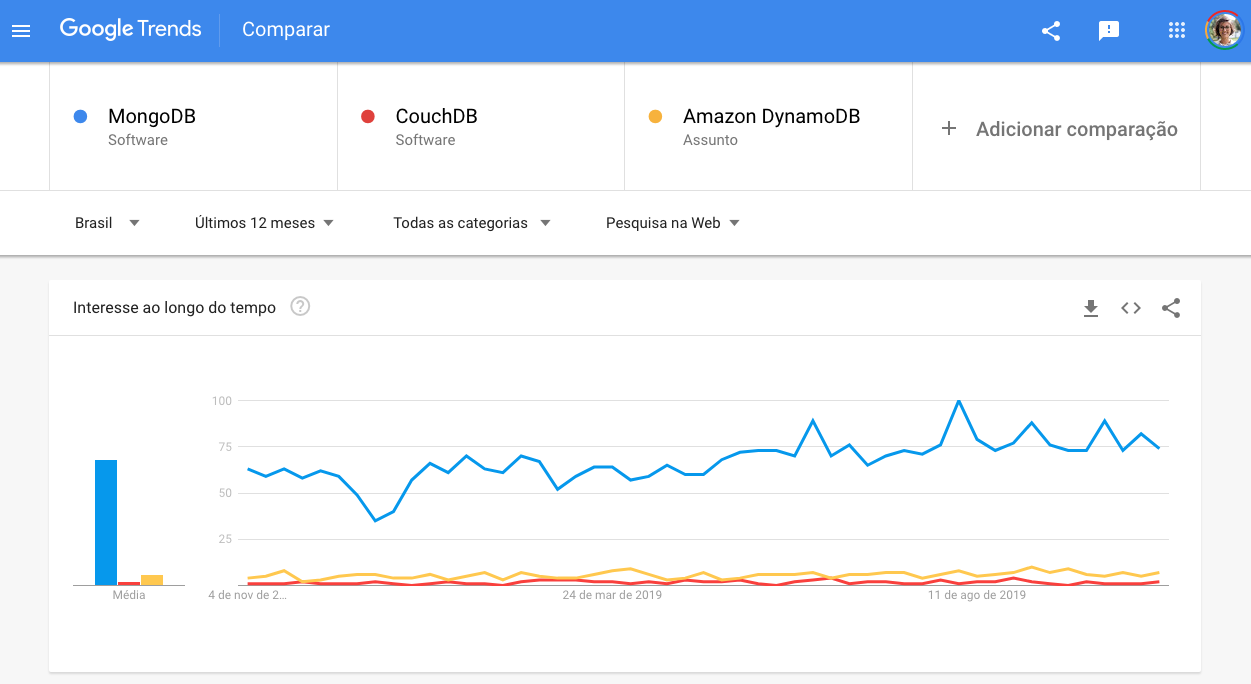
\includegraphics[width=400pt]{./imagens/trends.png}
	\caption{Popularidade do MongoDB em relação a outros DBs de documentos de acordo com o Google Trends 2019.}
	\label{plot:trends}
\end{figure}


\section{Padrões de modelagem NoSQL}
Pelo fato de um banco de dados de documentos ter a possibilidade de atuar sem um esquema (\textit{schemaless}), não significa que ele não poderá ter um esquema. E muito pelo contrário, os autores do MongoDB recomendam fortemente o uso de um esquema para modelar um banco de dados NoSQL, assim diminuindo os impactos da possível inconsistência de dados. 

Conforme a documentação \cite{mongodocs}, existem duas abordagens básicas, 1) Modelo de dados embutidos (MDE) (\textit{Embedded Data Models}), e 2) Modelo de dados normalizada (MDN) (\textit{Normalized Data Models}).

O \textbf{MDE} assume um formato de denormalização, onde o próprio documento contém as relações, e recomenda-se para quando há relações de um-para-muitos. Esta abordagem é execelente para recuperação de dados e também permite atualizar os dados relacionados em uma única operação atômica.

Em um \textbf{MDN}, as relações entre entidades são descritas usando referências para outros documentos através do atributo identificador, o ``{\under}id'', do documento referenciado. Esta abordagem é boa quando a duplicação de dados não está resultando ganhos performance na recuperação de dados. Também para representar relacionamentos muitos-para-muitos mais complexos. E para modelar grandes conjuntos de dados hierárquicos.

Além deste guia de modelagem básica, os autores do blog do MongoDB, disponibilizaram uma série de artigos sobre padrões de modelagem do banco de dados NoSQL. Um total de 12 padrões foram criados à partir do conhecimento adquirido na consultoria à clientes, é possível consultá-los rapidamente por uma matriz com o contexto de aplicação dos mesmos na figura \ref{plot:patternmatrix} \cite{mongoblogpatterns}.

Os padrões propostos não são excludentes, ou seja, é possível implementar mais de um padrão em uma solução. Portanto escolheu-se 4 destes padrões que contribuem à necessidade do uso dos dados com base nos requisitos funcionais. São eles:

\begin{enumerate}
  \item \textbf{\textit{Attribute Pattern}} (padrão de atributos): diminuí o indexamento de atributos parecidos, transportando-os para uma estrutura de lista;
  \item \textbf{\textit{Polymorphic Pattern}} (padrão polimórfico): o mesmo documento tem diferentes formatos porém compartilha de muitos atributos em comum. Então agrupa-se os documentos com base nas \textit{queries} (consultas) que necessitamos fazer. Com isto, ameniza-se a necessidade de fazer ``\textit{joins}'' (ligações) complexos;
  \item \textbf{\textit{Outlier Pattern}} (padrão fora da curva): usado quando o fator ``popularidade'' acontece, e um documento tem seu tamanho aumentado considerávelmente (por exemplo 16Mb). Para isto, cria-se um atributo ``\textit{flag}'' que sinalizará este fator em determinado documento e transportará os dados excedentes para um ou mais documentos (estes chamados de ``\textit{overflow documents}''), deixando apenas um número limitado no documento principal. Este padrão evita mudar todo um esquema por causa de um fato isolado;
  \item \textbf{\textit{The Computed Pattern}} (o padrão computado): quando temos dados que precisam ser computados repetitivamente, ou a partir de outros dados. Também serve para quando há mais leitura do que escrita de dados. Ótimo quando é necessário montar listas como ``100 melhores ...'';
  \item \textbf{\textit{Subset Pattern}} (padrão subconjunto): Quando o alocamento de memória RAM é alto devido ao tamanho dos documentos. Resulta em dados sendo removidos da memória RAM criando um subconjunto de dados menos usados (similar ao \textit{Outlier Pattern}).
\end{enumerate}

\begin{figure}[!htpb]
	\centering
	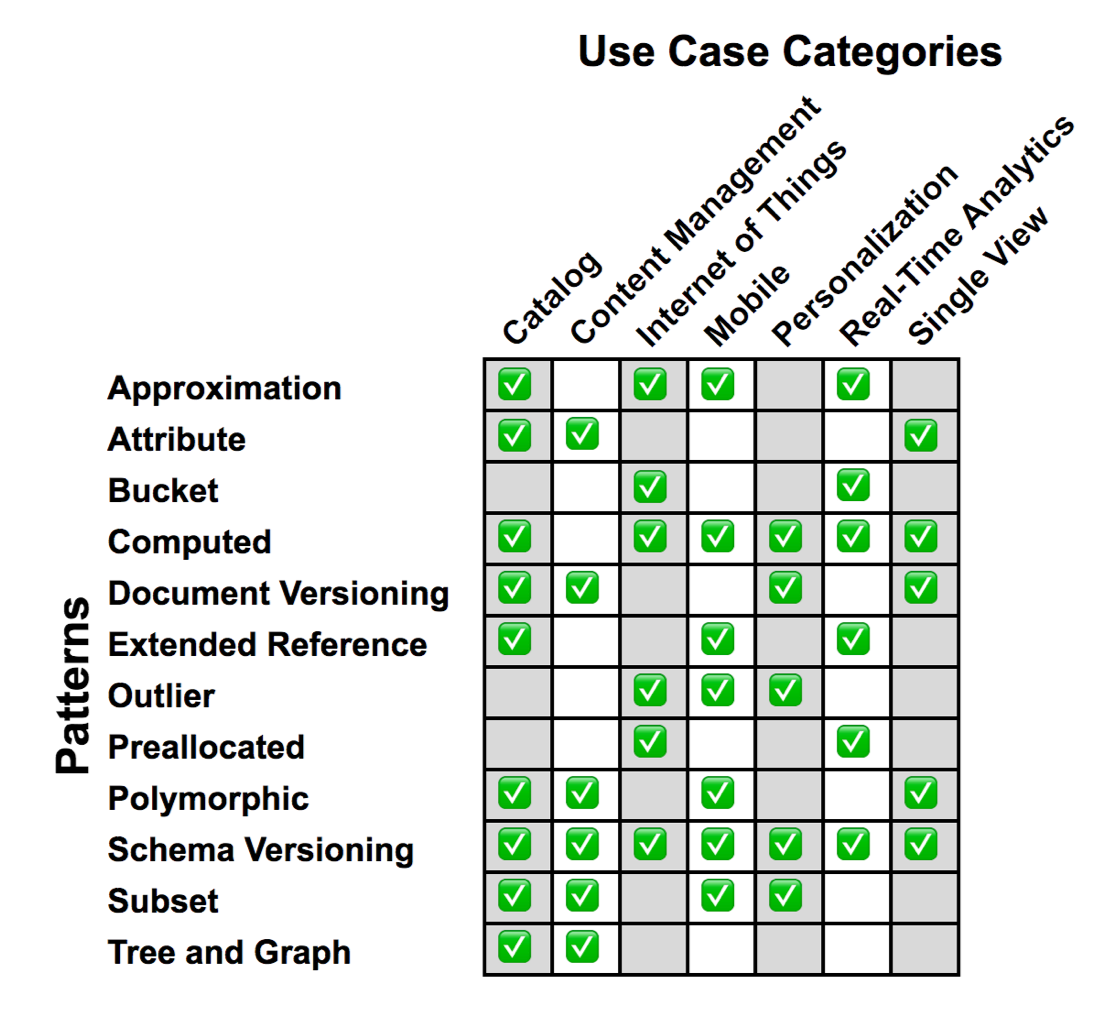
\includegraphics[width=300pt]{./imagens/patternsmatrix.png}
	\caption{Matriz de padrões de modelagem para o MongoDB}
	\label{plot:patternmatrix}
\end{figure}

\section{Unindo dados}
Mesmo sendo um banco de dados não relacional, em algumas situações se faz necessário o cruzamento de dados que estão em documentos diferentes, porém que guardam referência de um para o outro. Para isto o MongoDB oferece o \textbf{\textit{Aggregation Framework}} (AF). Com ele dados são transformados em etapas, passando por um \textit{pipeline}, onde o resultado de um estágio é o insumo (entrada) do estágio seguinte \cite{views-materializadas}. Neste \textit{pipeline}, podem ser utilizados um ou mais operadores de transformação de dados para obter o resultado necessário, com isto é possível atender muitos dos requisitos funcionais solicitados.

\section{Persistência Poliglota}
Para atender a demanda de buscas recursivas, como obter todas as sequências dos filmes, entre outras, será necessário usar um banco de dados de grafos. Porém para isto não é necessário manter dados em diferentes tipos de armazenamento. Para caso do banco de dados orientado a grafos \textbf{Neo4j}, é possível usar um conector do MongoDB e um "sincronizador" de base de dados, onde a partir dos dados enviados do MongoDB o Neo4j gera sua base, para que consultas com grafos sejam feitas \cite{neo4jMongo}.

Em \textit{Graph Operations with MongoDB}, \cite{graphoperator} demonstra como devemos modelar um banco de dados NoSQL com MongoDB com a intenção de realizar operações do AF que contém operadores para retornar grafos como o \verb+$graphLookup+. De acordo com o autor, o AF do MongoDB atende 75\% dos casos de operações com grafos.

% ---
% Finaliza a parte no bookmark do PDF
% para que se inicie o bookmark na raiz
% e adiciona espaço de parte no Sumário
% ---
\phantompart 
\chapter{Apresentação do modelo}

\section[Modelos]{Modelos}

Para este caso, adotou-se uma modelagem mais próxima ao MDE para os documentos que terão mais relacionamentos como \textbf{produção artística} e \textbf{artistas}. Para dados com menos relações, foi criados documentos separados para auxilio da aplicação que irá preencher os documentos maiores a partir da referência dos dados destes documentos.

Foram mapeados 6 entidades que representarão os documentos de primeiro nível, abaixo segue uma descrição curta de cada uma:

\begin{enumerate}
	\item \textbf{Produção}: contém os dados de uma produção artística, e as avaliações recebidas dos usuários;
	\item \textbf{Artista}: contém os dados dos artistas considerando suas múltiplas atuações nas produções artísticas;
	\item \textbf{Produtora}: contém nome e país de uma produtora;
	\item \textbf{Generos}: contém o nome do gênero de uma produção artística, armazenando em si as referências das produções deste gênero, além de definir se é gênero musical ou cinematográfico; 
	\item \textbf{Usuário}: contém o registro de usuários cadastrados no site e a lista de avaliações feitas;
	\item \textbf{Resenhas}: contém o conteúdo criado por usuários privilegiados.
\end{enumerate}

\section[Descrição]{Descrição da modelagem}

Nesta sessão, a descrição das entidades mais complexas são detalhadas, e também observações adotadas nas demais entidades.

\subsection{Produção}
A entidade \textbf{Produção} representa seu respectivo documento no banco de dados, para a mesma, usou-se o padrão polimórfico, onde existe a flexibilidade de preencher o documento com os dados de um filme, ou uma série, ou caso ambos atributos não sejam preenchidos, os atributos contemplam os requisitos para um videoclipe. Porém é declarado o atributo \verb+tipo+ para armazenar o tipo de produção. O polimorfismo deste documento está representado pelo retângulo lilás no Diagrama de Entidades.

A entidade \textbf{Produção} do tipo \textbf{Filme} contém um atributo \verb+sequencia+, este representa a sequência de um série de filmes. Para que possa ser solicitado a sequência de um filme é armazenado a ordem que este filme está na sequência, além das referências do seu filme antecessor e sucessor, todos os dados da sequência são opcionais, sendo necessário atualizar por aplicação caso um sucessor seja inserido depois.

Tanto em \textbf{Filme} quanto em uma \textbf{Série} o atributo \verb+personagens+ armazena uma lista de documentos representados pela entidade \textbf{Personagens}, que por sua vez contém o nome dos personagens e a referência a seu respectivo artista.

Em \textbf{Filme} e em um \textbf{Episódio} de uma \textbf{Série}, o atributo \verb+avaliacaoArtista+  armazena uma lista de subdocumentos tendo seu modelo representado pela entidade \textbf{AvaliacaoArtista}, onde armazena os dados de avaliação da atuação dos artistas nesta produção, feitas pelos usuários do site. Cada avaliação de um artista é armazenada no atributo \verb+avaliacao+, que por sua vez recebe uma lista de documentos do tipo \textbf{Avaliacao} com a referência do usuário e a nota da atuação do artista. A referência da avaliação também deve ser gravada no documento do usuário autor da avaliação.

Na entidade \textbf{Episódio}, está previsto o cenário de artistas convidados, possibilitando que estes também possam receber avaliações da sua participação especial.

Ainda em uma \textbf{Produção}, é possível receber avaliações detalhadas dos usuários com um comentário. Portanto no atributo \verb+avaliacaoDosUsuarios+ é armazenado uma lista de documentos do tipo \textbf{AvaliacaoDosUsuarios}. O comentário de uma avaliação pode receber uma nota também, portanto um comentário é um subdocumento do tipo \textbf{Comentario}, onde guarda no atributo \verb+avaliacao+ que contém uma lista de documentos do tipo \textbf{Avaliacao}.

O atributo \verb+popular+ de uma \textbf{Produção} faz um papel de \textit{flag}, ou sinalização, se a determinada produção é popular, isto é um indicador para adotar o padrão fora da curva, para armazenar um numero menor de avaliações e o maior volume em um documento separado.

\subsection{Artista}
O documento que armazenará os detalhes dos artistas, bandas e diretores é o \textbf{Artista}. Este documento contém atributos simples, apenas uma observação que em seu subdocumento \verb+atuacaoTipo+ é definido se um artista é multifacetado ou uma grupo musical, seguindo o padrão de atributos.

\subsection{Atributos de média de nota}
Os atributos das entidades que armazenarão uma média de nota de avaliação das produções artísticas ou de artistas, serão preenchidos de maneira computada por uma função do banco de dados, fazendo o \verb+reduce+ (soma) de todas as notas e dividindo pelo tamanho da lista que armazena estas notas. Esta função deverá ser disparada a cada nova avaliação feita. Esta possibilidade se dá pela implementação do padrão computado.

\subsection{Chaves primárias}
As chaves primárias artificiais são geradas automaticamente pelo sistema de banco de dados no momento em que o documento é inserido. Estes documentos recebem uma chave com o nome ``{\under}id'' onde esta já vem as regras de unicidade, e uma hash é gerada pela função \verb+ObjectId()+, estas chaves foram omitidas de declaração no Diagrama de Entidades.

\subsection{Demais entidades} 
As demais entidades são simples, e algumas, como \textbf{Produtora} e \textbf{Generos} são para ajudar a manter uma consistência de dados no preenchimento dos campos de outras entidades.

%\textbf{}
%\verb++

\newgeometry{margin=1cm}
\begin{landscape}
\thispagestyle{empty} %% Remove header and footer.
\tikzumlset{font=\tiny\ttfamily}
\begin{center}
	\textbf{Diagrama de Entidades}
\end{center}
\begin{tikzpicture}

	% entidades
		% pacote producao
		\begin{umlpackage}{ProducaoDocumento} 
			\umlclass[x=0,y=-1.7]{Producao}{  
				titulo: string \\ 
				resumo: string \\ 
				enredo: string \\
				cadastradoPor: string \\
				generos: string[] \\
				videoTrailer: string \\
				capa: string \\
				tipo: string \\
				ano: int32 \\
				duracao: int32 \\
				classificacaoEtaria: int32 \\
				mediaAvaliacao: int32 \\
				popular: boolean \\
				filme: document \\
				serie: document \\
				paisesProdutores: string[] \\
				produtorasId: string[] \\
				estreandoArtistaId: string[] \\
				diretoresId: string[]\\
				avaliacaoDosUsuarios: document[]\\
			}{}
	
			\umlclass[x=7,y=0]{Filme}{  
				bilheteria: int32 \\ 
				faturamento: int32 \\ 
				sequencia: document \\ 
				personagens: document[] \\
				avaliacaoArtista: document[] \\
			}{}

			\umlclass[x=7,y=-4]{Serie}{  
				qtdTemporadas: int32 \\
				personagens: document[] \\
				episodios: document[]
			}{}
		\end{umlpackage}
	
		\umlclass[x=13,y=2]{Sequencia}{  
			ordem: int32 \\ 
			antecessorId: string \\ 
			sucessorId: string \\ 
		}{}

		\umlclass[x=13,y=-2]{Personagens}{  
			nome: string \\ 
			atuadoPorId: string \\ 
		}{}

		\umlclass[x=18,y=0]{AvaliacaoArtista}{  
			artistaId: string \\ 
			mediaAvaliacao: int32 \\ 
			avaliacao: document[] \\ 
		}{}

		\umlclass[x=23,y=0]{Avaliacao}{  
			usuarioId: string \\ 
			nota: int32 \\ 
		}{}

		\umlclass[x=15,y=-7]{Episodio}{  
			numero: int32 \\
			temporada: int32 \\
			temporadaNome: string\\
			atoresConvidadosId: string[] \\
			diretoresConvidadosId: string[] \\
			personagensConvidados: document[] \\
			avaliacaoArtista: document[] \\
		}{}

		\umlclass[x=0,y=-8.8]{AvaliacaoDosUsuarios}{  
			data: date \\
			usuarioId: string \\
			producaoId: string \\
			nota: int32 \\
			comentario: document
		}{}

		\umlclass[x=0,y=-12.5]{Comentario}{  
			conteudo: string \\
			mediaAvaliacao: int32 \\
			avaliacao: document[]
		}{}
	
		\umlclass[x=22,y=-4]{Artista}{  
			nome: string \\
			miniBiografia: string \\
			dataDeObito: date \\
			dataDeNascimento: date \\
			localDeNascimento: string \\
			atuouEmId: string[] \\
			atuacaoTipo: document \\
		}{}

		\umlclass[x=22,y=-8.5]{AtuacaoTipo}{  
			musical: boolean \\
			cinema: boolean \\
			direcao: boolean \\
			grupoMusical: boolean \\
		}{} 
		
		\umlclass[x=6.5,y=-11]{Usuario}{  
			nome: string \\
			sobrenome: string \\
			nomeDeUsuario: string \\
			email: string \\
			senha: string \\
			cidade: string \\
			mediaAvaliacao: int32 \\
			usuarioPrivilegiado: boolean \\ 
			avaliacoesFeitasId: string[] \\
		}{}

		\umlclass[x=11.5,y=-12]{Produtora}{  
			nome: string \\
			pais: string \\
		}{}

		\umlclass[x=16,y=-12]{Generos}{  
		}{
			nome: string \\ 
			producoesId: string[] \\ 
			tipo: string \\ 
		}

		\umlclass[x=21	,y=-12]{Resenhas}{  
		}{
			titulo: string \\
			data: date \\
			usuarioAutorId: string \\
			resumo: string \\
			conteudo: string \\
		}

		\umlunicompo[geometry=-|-, mult1=1, mult2=0]{Producao}{Filme} 
		\umlunicompo[geometry=-|-, mult1=1, mult2=0]{Producao}{Serie}
		\umlunicompo[mult1=1, mult2=*]{Producao}{AvaliacaoDosUsuarios}
		\umlunicompo[mult1=1, mult2=1]{AvaliacaoDosUsuarios}{Comentario}

		\umlunicompo[mult1=1, mult2=1]{Filme}{Sequencia}
		\umlunicompo[mult1=1, mult2=*]{Filme}{Personagens}
		\umlunicompo[mult1=1, mult2=*]{Filme}{AvaliacaoArtista}
		\umlunicompo[mult1=1, mult2=*]{AvaliacaoArtista}{Avaliacao}
		
		\umlunicompo[mult1=1, mult2=*]{Serie}{Personagens}
		\umlunicompo[mult1=1, mult2=*]{Serie}{Episodio}
		\umlunicompo[mult1=1, mult2=*]{Episodio}{Personagens}
		\umlunicompo[mult1=1, mult2=*]{Episodio}{AvaliacaoArtista}

		\umlunicompo[mult1=1, mult2=1]{Artista}{AtuacaoTipo}


	\end{tikzpicture}
\end{landscape}
\restoregeometry

% ----------------------------------------------------------
% ELEMENTOS PÓS-TEXTUAIS
% ----------------------------------------------------------
\postextual


% ----------------------------------------------------------
% Referências bibliográficas
% ----------------------------------------------------------


\nocite{MFnosql}
%\nocite{MFpolyglot}
\nocite{graphoperator}
\nocite{DMleftJoin}
\nocite{mongopolyglot}
\bibliography{modelagem-nosql}



\end{document}
